\section{Solidity to Control-Flow Graph}

Here we describe how we model Solidity programs as control-flow graphs. First we discuss how to model individual functions, in Section \ref{sec:sol_cfg_fun}, and then, in Section \ref{sec:sol_cfg_con}, the general approach for modelling a whole contract is presented.

%%%%%%%%%%%%%%%%%%%%%%%%%%%%%%%%%%%%%%%%%%

\subsection{Control-Flow Graph of a Solidity Function} \label{sec:sol_cfg_fun}

To generate the control-flow graph of a Solidity function we initially create an entry node to represent its start. Beginning from the entry node, the code is scanned until the function ends or a return statement is reached. During the scanning process, statements that do not influence the control-flow, such as assignments, are stored in the current node for future analysis. When control structures are reached, however, the graph is updated according to their semantics. To model the end of the function, a sink, called the exit node, is created, being the targeted by every node with a return statements, and if none exist, by node storing the last statement of the function.

The shape of the resulting graph depends of the control structures present in the function. The graphs generate by some common structures can be seen inside the dotted squares in figures \ref{fig:cfg_if}, \ref{fig:cfg_if-else}, and \ref{fig:cfg_while}; the edges with no tag have value \texttt{true}. Each condition generates an empty node with two outward edges, one with the condition itself, and one with its negation. Control structures can be combined to model complex scenarios, such as nested loops.

The encoding of the Solidity assertions is done according to their semantics. The \texttt{require} operator works as a pre-condition, and is thus simply added inside the current node. The \texttt{assert} operator works as a post-condition, and is encoded as a conditional with the \texttt{then} branch targeting the next node in the graph, and the \texttt{else} branch targeting the error node. The error node is a special sink node in our model, and reaching it represents an error in the execution. The graph representing an \texttt{assert} can be seen in Figure \ref{fig:cfg_assert}.

\begin{figure}[ht]
  \centering
  \begin{minipage}[h]{0.45\textwidth}
  	\centering
    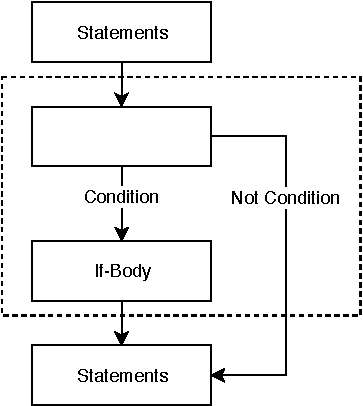
\includegraphics[width=0.7\textwidth]{images/if}
    \caption{Graph of the if-then}
    \label{fig:cfg_if}
  \end{minipage}
  \hfill
  \begin{minipage}[h]{0.45\textwidth}
  	\centering
    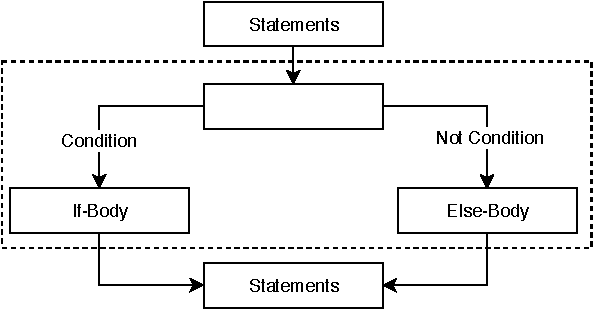
\includegraphics[width=\textwidth]{images/if-else}
    \caption{Graph of the if-then-else}
    \label{fig:cfg_if-else}
  \end{minipage}
  \newline \newline \vfill
  \begin{minipage}[h]{0.45\textwidth}
  	\centering
    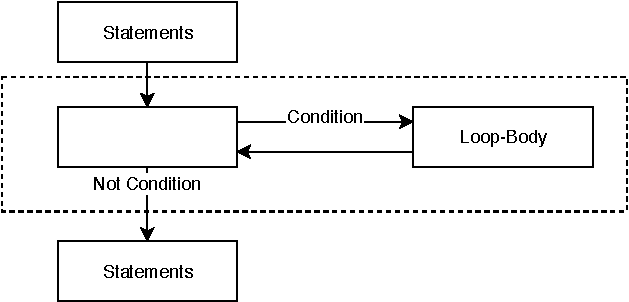
\includegraphics[width=\textwidth]{images/while}
    \caption{Graph of the while-loop}
    \label{fig:cfg_while}
  \end{minipage}
  \hfill
  \begin{minipage}[h]{0.45\textwidth}
  	\centering
    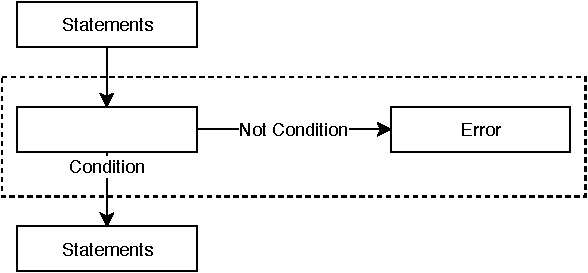
\includegraphics[width=\textwidth]{images/assert}
    \caption{Graph of the assert}
    \label{fig:cfg_assert}
  \end{minipage}
\end{figure}

The control-flow graph of \texttt{average} function shown in Section \ref{sec:background_sol} can be seen in Figure \ref{fig:cfg_average}. In this example we can see that the variables \texttt{count} and \texttt{sum} are used but not defined, since they are state variables; the return variable is initialized with its default value. To correctly encode state variables, a model of the whole contract is required.

\begin{figure}[ht]
	\centering
	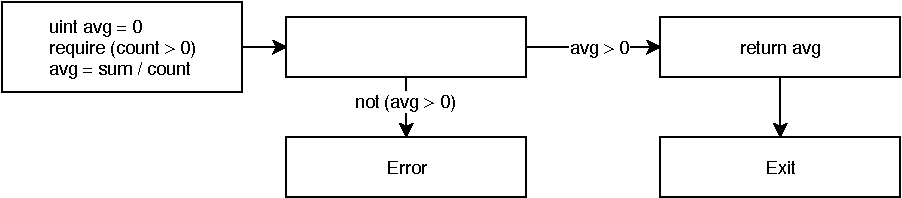
\includegraphics[width=0.7\textwidth]{images/average}
	\caption{Graph of the average function}
	\label{fig:cfg_average}
\end{figure}

%%%%%%%%%%%%%%%%%%%%%%%%%%%%%%%%%%%%%%%%%%

\subsection{Control-Flow Graph of a Solidity Contract} \label{sec:sol_cfg_con}

Unlike programming languages such as C++ and Java, Solidity does not have a main function, the functions of a given contract can be called independently and in any order. To capture the behaviour of a whole contract in a single control-flow graph, we create an infrastructure to model calls to functions, as can be seen in Figure \ref{}.

The entry node of the graph models the constructor of the contract, which is a special function that is executed before deploying the contract on the blockchain, with the goal of initializing state variables. From the constructor only one transition is possible, to the interface node, which is an internal node that targets the entry node of each function in the contract. To represent the fact that the contract functions can be called in any order, the transitions starting at the interface are nondeterministic, with their predicates being simply "true". To allow for many function calls, the exit node of each function targets the interface node.

The final point to consider is the use of assertions. The \texttt{require} operator is handled as previously described, since it does not influence the control-flow. The \texttt{assert} operator, however, now targets a global error state, instead of a specific one for each function. This change makes checking the contract easier, since we only need verify if one particular state can be reached. 